\documentclass[11pt]{article}
\usepackage[margin=0.9in]{geometry}\usepackage{graphicx,booktabs,amsmath,float}
\title{Does the Prior Help when Data is Scarce? Ill-Posed Image-Space Supervision}
\author{Patient-Specific Residual INR --- SLAM Ax\_T2\_2D, change\_extent=1}
\date{\today}\begin{document}\maketitle
\section*{Setup}
We reconstruct a single follow-up slice from only a subset of its pixels, to probe the regime that actually matters for accelerated MRI: \emph{insufficient} data. The residual (or, for baselines, the reconstruction) is supervised only on the observed pixels and evaluated on the \emph{full} image. Four methods share the same observed pixels: \textbf{current-only INR} (no prior, the robust floor); \textbf{prior-finetune} (NeRP-style, the prior INR fine-tuned on observed pixels); \textbf{ours} (frozen prior + residual); and \textbf{ours+gate} (adds a spatial trust gate). If the prior is worth its keep, the prior-anchored methods should hold up as supervision shrinks while current-only collapses.
\subsection*{A. Very sparse random supervision}
A random fraction $p$ of pixels is observed (scattered across the image), swept from 50\% down to 2\%. As $p$ falls the gaps between observed pixels grow, so pure interpolation (current-only) degrades; a prior can fill the gaps with plausible anatomy.
\begin{table}[H]\centering\caption{Very sparse random: full-image metrics vs.\ observed fraction $p$.}
\begin{tabular}{llrrr}\toprule
$p$ & method & PSNR & SSIM & change-gain \\ \midrule
50\% & current-only INR & 32.11 & 0.914 & 0.977 \\
 & prior-finetune (NeRP) & 32.44 & 0.925 & 0.975 \\
 & \textbf{prior+residual (ours)} & 28.44 & 0.813 & 0.883 \\
 & \textbf{prior+gated residual (ours+gate)} & 29.05 & 0.904 & 0.904 \\
\midrule
25\% & current-only INR & 28.48 & 0.846 & 0.953 \\
 & prior-finetune (NeRP) & 29.15 & 0.873 & 0.942 \\
 & \textbf{prior+residual (ours)} & 25.37 & 0.763 & 0.776 \\
 & \textbf{prior+gated residual (ours+gate)} & 25.64 & 0.839 & 0.785 \\
\midrule
10\% & current-only INR & 24.41 & 0.766 & 0.925 \\
 & prior-finetune (NeRP) & 25.72 & 0.799 & 0.872 \\
 & \textbf{prior+residual (ours)} & 22.60 & 0.695 & 0.613 \\
 & \textbf{prior+gated residual (ours+gate)} & 22.32 & 0.739 & 0.566 \\
\midrule
5\% & current-only INR & 22.24 & 0.692 & 0.898 \\
 & prior-finetune (NeRP) & 24.19 & 0.724 & 0.807 \\
 & \textbf{prior+residual (ours)} & 21.54 & 0.679 & 0.506 \\
 & \textbf{prior+gated residual (ours+gate)} & 21.31 & 0.718 & 0.429 \\
\midrule
2\% & current-only INR & 20.27 & 0.565 & 0.951 \\
 & prior-finetune (NeRP) & 22.81 & 0.571 & 0.720 \\
 & \textbf{prior+residual (ours)} & 20.78 & 0.619 & 0.415 \\
 & \textbf{prior+gated residual (ours+gate)} & 20.57 & 0.698 & 0.351 \\
\bottomrule\end{tabular}\end{table}
\begin{figure}[H]\centering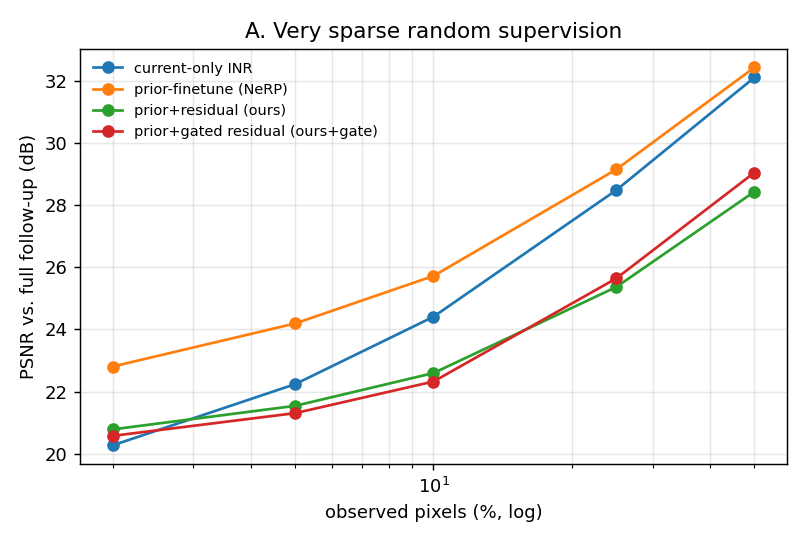
\includegraphics[width=0.62\linewidth]{curveA.png}
\caption{PSNR vs.\ observed fraction (log axis). A flat curve = robust to data scarcity.}\end{figure}
\begin{figure}[H]\centering
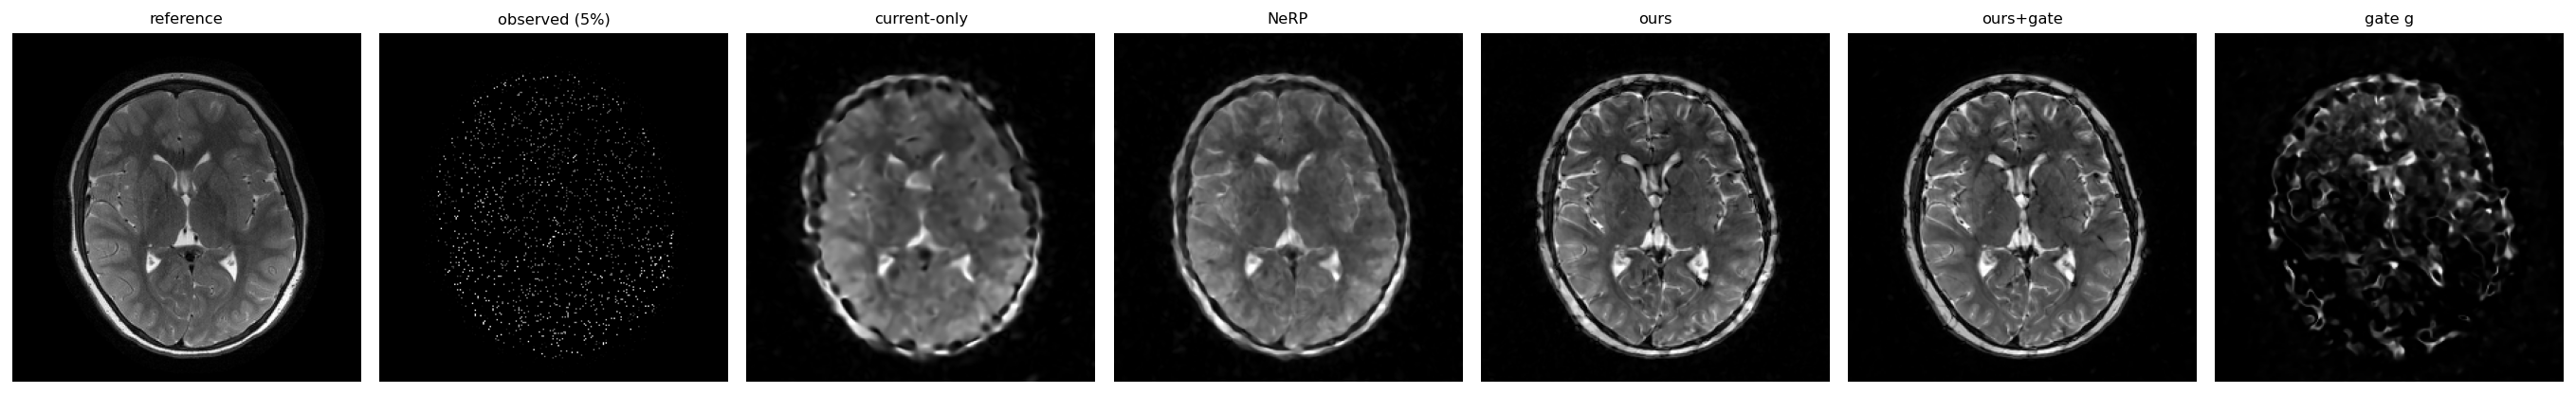
\includegraphics[width=\linewidth]{panelA_p005.png}
\caption{Reconstructions at $p=5\%$: reference, observed pixels, then each method, and the gate map (white = distrust prior).}
\end{figure}
\subsection*{B. Structured hole}
Everything is observed \emph{except} a central square hole of side $h$; the hole has no interior samples, so it can only be filled by extrapolation or from the prior. As $h$ grows the reconstruction inside the hole depends entirely on the prior.
\begin{table}[H]\centering\caption{Structured hole: PSNR inside the hole (the filled region) and over the full image.}
\begin{tabular}{llrrr}\toprule
hole $h$ & method & PSNR(hole) & PSNR(full) & SSIM(full) \\ \midrule
0 & current-only INR & 38.95 & 38.95 & 0.961 \\
 & prior-finetune (NeRP) & 46.64 & 46.64 & 0.989 \\
 & \textbf{prior+residual (ours)} & 34.95 & 34.95 & 0.898 \\
 & \textbf{prior+gated residual (ours+gate)} & 37.44 & 37.44 & 0.977 \\
\midrule
48 & current-only INR & 16.61 & 30.44 & 0.936 \\
 & prior-finetune (NeRP) & 20.46 & 34.68 & 0.965 \\
 & \textbf{prior+residual (ours)} & 16.31 & 29.53 & 0.890 \\
 & \textbf{prior+gated residual (ours+gate)} & 16.23 & 30.00 & 0.961 \\
\midrule
96 & current-only INR & 13.91 & 22.33 & 0.845 \\
 & prior-finetune (NeRP) & 19.20 & 27.66 & 0.893 \\
 & \textbf{prior+residual (ours)} & 16.00 & 24.26 & 0.850 \\
 & \textbf{prior+gated residual (ours+gate)} & 15.93 & 24.29 & 0.911 \\
\midrule
144 & current-only INR & 12.83 & 17.80 & 0.702 \\
 & prior-finetune (NeRP) & 18.63 & 23.61 & 0.782 \\
 & \textbf{prior+residual (ours)} & 16.20 & 21.14 & 0.789 \\
 & \textbf{prior+gated residual (ours+gate)} & 16.07 & 21.04 & 0.831 \\
\bottomrule\end{tabular}\end{table}
\begin{figure}[H]\centering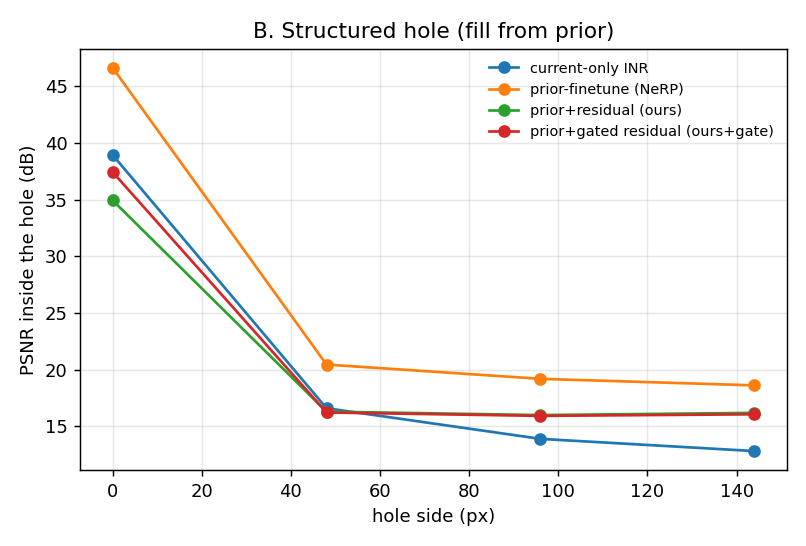
\includegraphics[width=0.62\linewidth]{curveB.png}
\caption{PSNR inside the hole vs.\ hole size. current-only cannot fill a hole it never saw.}\end{figure}
\begin{figure}[H]\centering
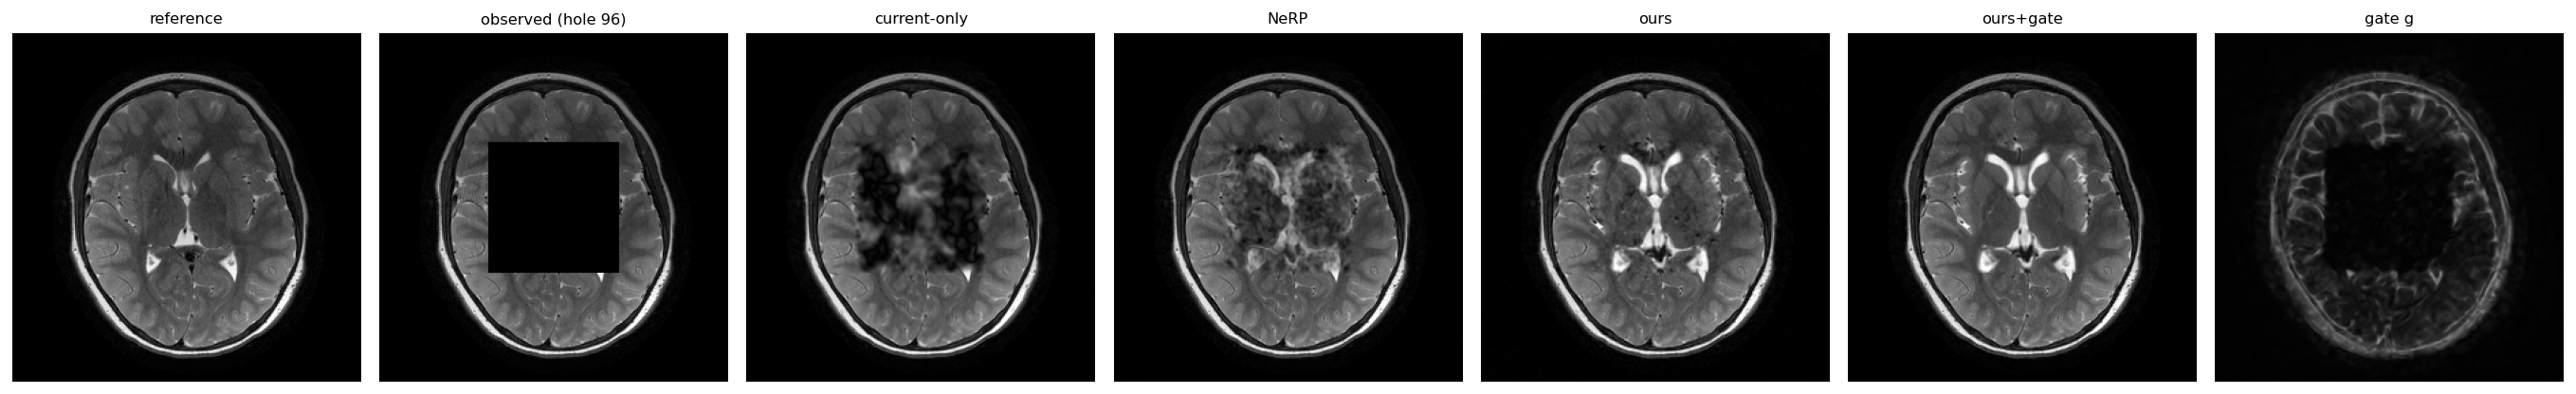
\includegraphics[width=\linewidth]{panelB_h096.png}
\caption{Reconstructions with a 96px hole: reference, observed (hole blanked), then each method, and the gate map.}
\end{figure}
\end{document}